\section{Deep learning fundamentals}

Deep learning has emerged as a powerful subset of machine learning,
revolutionizing the field of artificial intelligence. Its roots can
be traced back to the early development of artificial neural networks
in the 1940s and 1950s, with significant milestones including the
perceptron in 1958 and the backpropagation algorithm in the 1980s.
However, it wasn't until the early 21st century, with the advent of
more powerful computational resources and the availability of large
datasets, that deep learning truly began to flourish.

\subsection{Learning Paradigms}

Deep learning systems can be categorized into three main learning paradigms.
The most common approach is supervised learning, where models learn from
labeled data by mapping inputs to known outputs. This paradigm requires a
large amount of labeled training data, which can be expensive and
time-consuming to acquire. Semi-supervised learning offers a hybrid
approach that leverages both labeled and unlabeled data, proving
particularly useful when labeled data is scarce but unlabeled data is
abundant. Finally, unsupervised learning enables models to discover
patterns and structures from unlabeled data without explicit guidance,
making it valuable for tasks like clustering and dimensionality
reduction.

\subsection{Architecture and Training}

Deep learning architectures are characterized by their layered
structure, where each layer progressively extracts and transforms
features from the input data. The early layers typically focus on
low-level feature extraction, such as edges, textures, and basic
patterns in the case of image processing. As information flows through
the network, middle layers combine these basic features into more
complex representations. The final layers perform high-level reasoning
and make the ultimate predictions or classifications.

The training process relies heavily on the gradient descent
algorithm, which iteratively adjusts the model's parameters to
minimize a loss function. This loss function serves as a crucial
component of the learning process, quantifying how well the model's
predictions match the actual targets. By providing a measure of the
model's performance, the loss function guides the optimization process,
enabling the network to learn meaningful patterns from the training
data.

\subsection{Challenges and Solutions}

Despite their power, deep learning systems face several significant
challenges. One of the most prominent issues is overfitting, where
models may memorize training data instead of learning generalizable
patterns. This challenge is typically addressed through various
regularization techniques such as dropout, L1/L2 regularization, and
early stopping. Another critical challenge is the substantial data
requirements; deep learning models often need massive amounts of
training data to achieve good performance, which can be a limiting
factor in many applications. Additionally, the complex, layered nature
of deep learning models makes them difficult to interpret, often
referred to as "black boxes." This lack of transparency can be
particularly problematic in critical applications where understanding
the decision-making process is essential.

\subsection{Deep Learning Frameworks}

The development of powerful open-source frameworks has significantly
accelerated deep learning research and applications. TensorFlow,
developed by Google, provides a comprehensive ecosystem for building
and deploying machine learning models. PyTorch, created by Facebook's AI
Research lab, offers dynamic computation graphs and has become
particularly popular in research settings. Caffe, known for its speed
and modularity, is widely used in computer vision applications.

These frameworks have democratized deep learning by providing
efficient implementations of common operations, automatic
differentiation for gradient computation, and GPU acceleration for
faster training. They also offer pre-trained models and transfer
learning capabilities, along with active communities for support and
knowledge sharing. The combination of these frameworks with modern
hardware has enabled researchers and practitioners to develop
increasingly sophisticated models, pushing the boundaries of what's
possible in artificial intelligence. As shown in
Figure~\ref{fig:dl_frameworks_trends}, which presents data from
Google Trends over the last five years (as of April 2025), TensorFlow
and PyTorch have emerged as the two most prominent frameworks in the
deep learning landscape.

\begin{figure}[h]
  \centering
  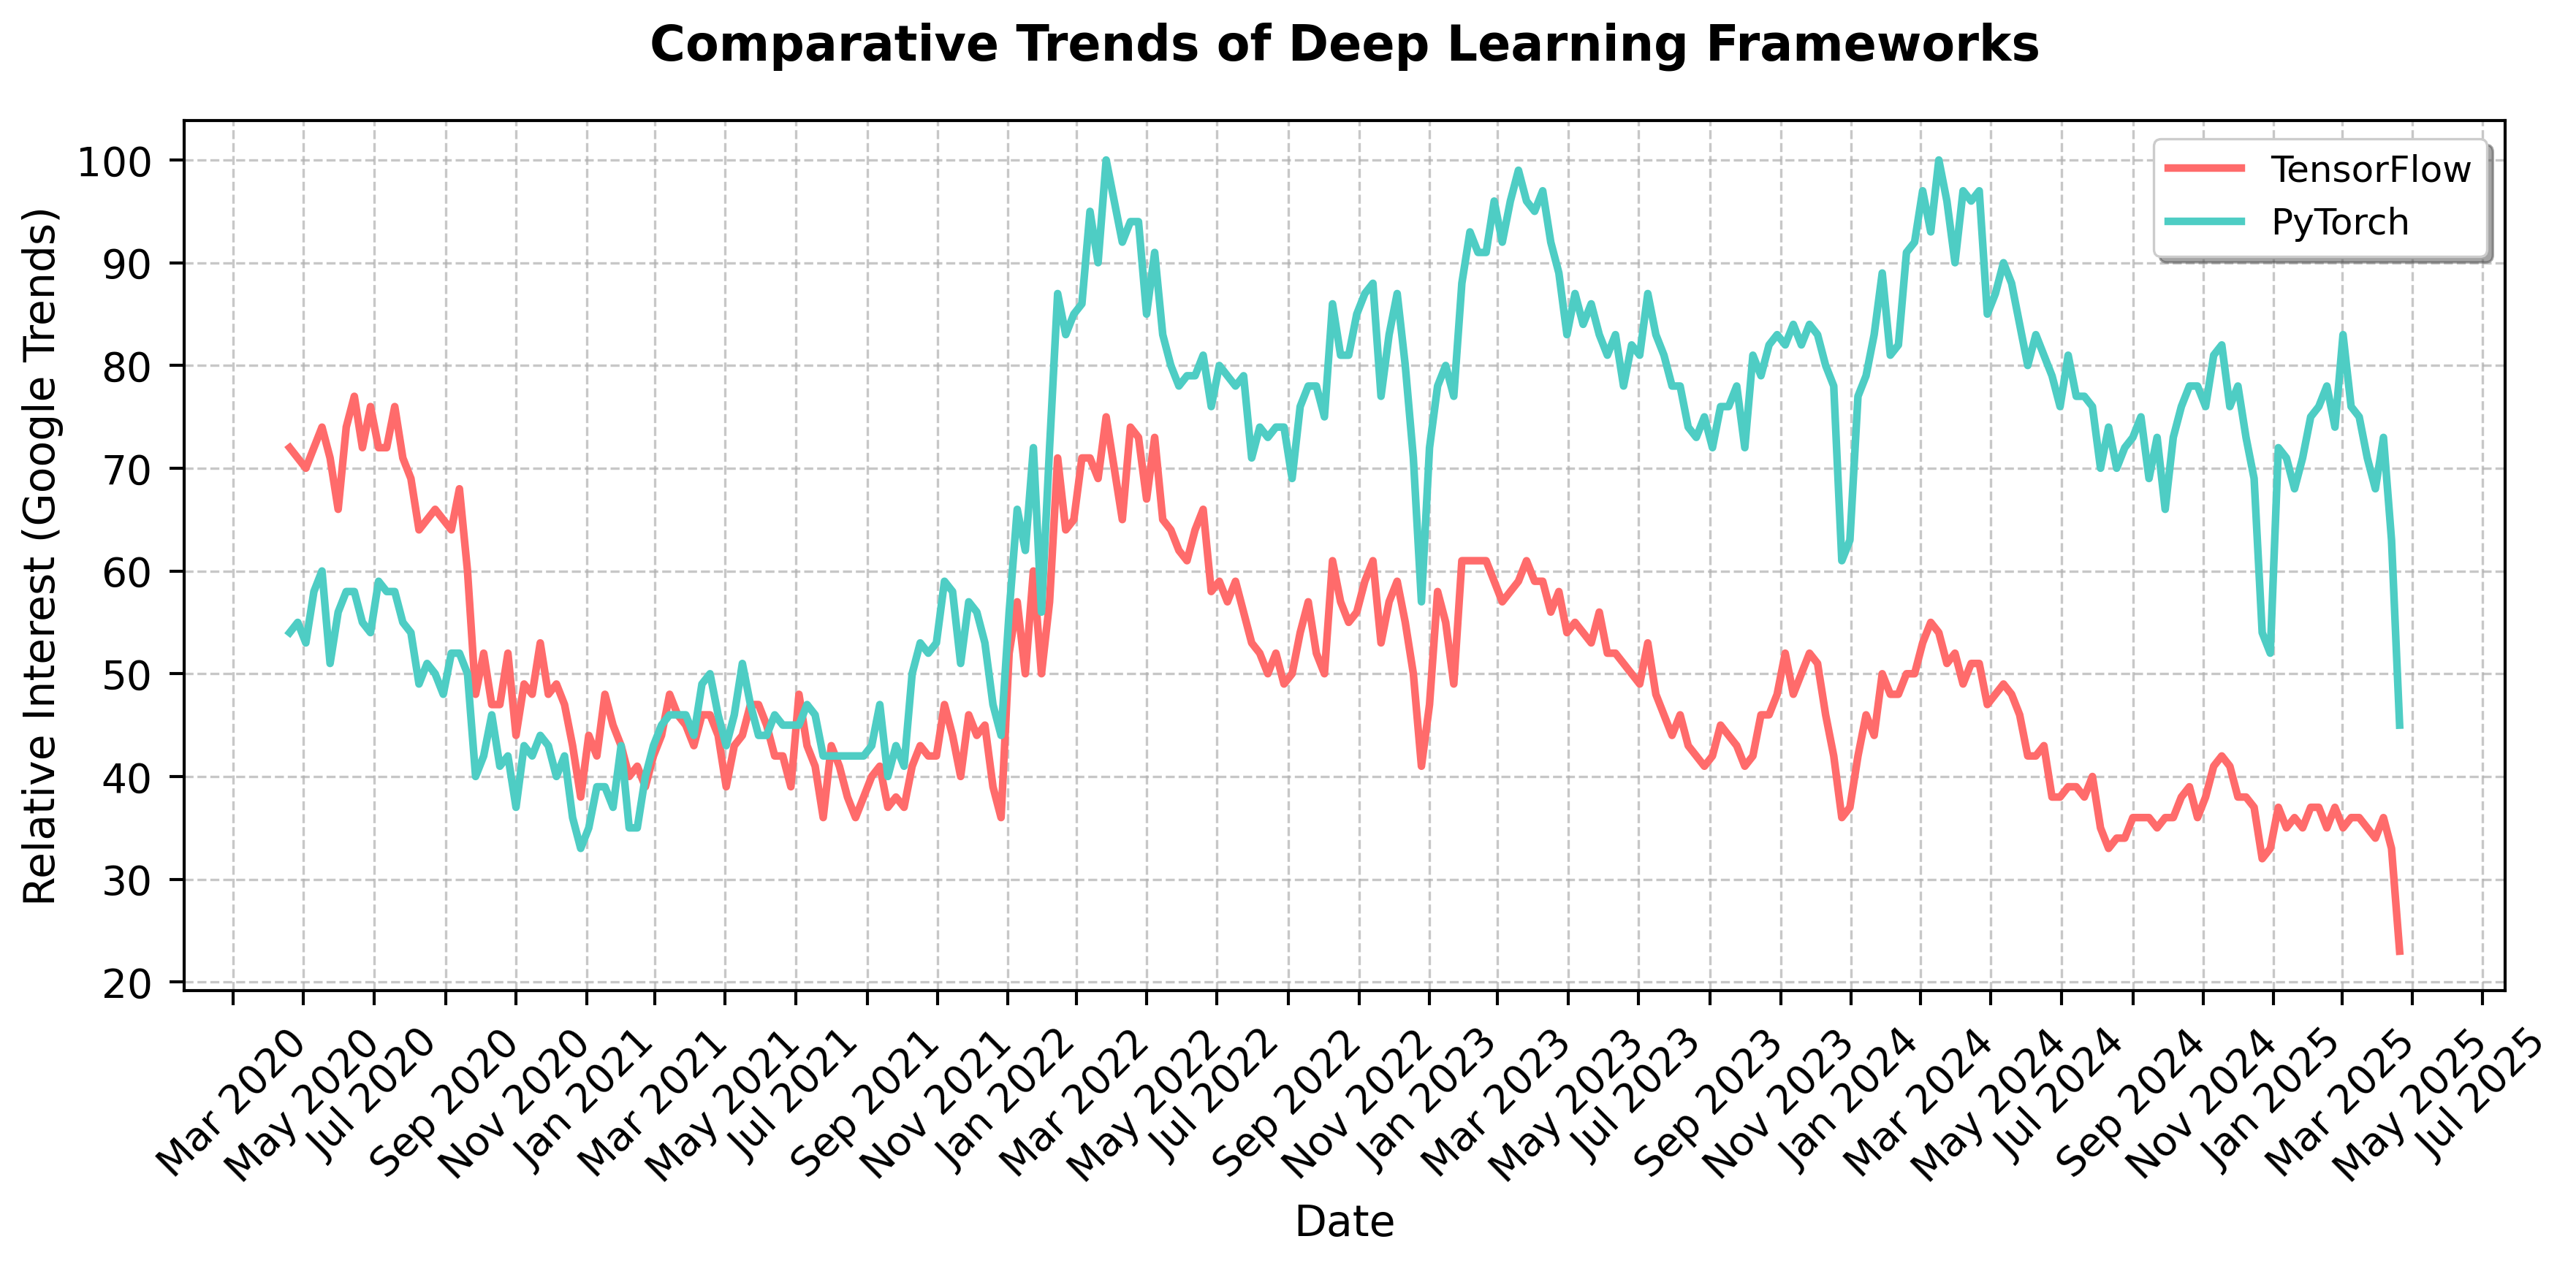
\includegraphics[width=0.8\textwidth]{Cap2/Figures/dl_frameworks_trends.png}
  \caption{Comparative Trends of the top two most popular Deep
  Learning Frameworks, apparently, tendency was switched to PyTorch since 2022}
  \label{fig:dl_frameworks_trends}
\end{figure}
